\documentclass[12pt]{article}

\setlength{\parindent}{0pt}
\setlength{\parskip}{2mm}

\usepackage{geometry}
 \geometry{
 letterpaper, left=20mm, right=20mm,  top=20mm,
 }
\usepackage{graphicx}
\graphicspath{ {graphics/} }
\usepackage{amssymb}
\usepackage[hidelinks]{hyperref}
\usepackage{wrapfig}
\usepackage[margin=1.2cm]{caption}
\usepackage{intcalc}


%%%%%%%%%%%%%%%%%%% TIKZ CUSTOM SHAPES AND SETTINGS
\usepackage{tikz}
\usetikzlibrary{shapes.geometric}
\usetikzlibrary{arrows}
\usetikzlibrary{positioning}
\tikzstyle{hydrophone} = [draw, circle, radius=5mm]
%%%%%%%%%%%%%%%%%%%%%%%%%%%%%%%%%%%%%%%%%%%%%%%%%%%%%%%%%%%%%%%%%%%%%%%%%%%%%%%


%%%%%%%%%%%%%%%%%%%%%%%%%%%%%%%%%%%%%%%%%%%%%%%%%%%%%%%%%%%%%%%%%%%%%%%%%%%%%%%
\begin{document}

%%%%%%%%%%%%%%%%%%%%%%%%%%%%%%%%%%%%%%%%%%%%%%%%%%%%%%%%%%%%%%%%%%%%%%%%%%%%%%%
\begin{titlepage}

\vspace*{5cm}

\begin{huge}
Setup and User Guide
\end{huge}

\begin{large}
Crab Tracker

\vspace*{1cm}

\textbf{Noah Strong}

\vspace*{1cm}
\end{large}

\textit{Revision 1.0-WIP}\\
\today

\vfill
\hfill 
\includegraphics[scale=1]{ct-logo.png}

\end{titlepage}
%%%%%%%%%%%%%%%%%%%%%%%%%%%%%%%%%%%%%%%%%%%%%%%%%%%%%%%%%%%%%%%%%%%%%%%%%%%%%%%
\tableofcontents{}

\newpage

%%%%%%%%%%%%%%%%%%%%%%%%%%%%%%%%%%%%%%%%%%%%%%%%%%%%%%%%%%%%%%%%%%%%%%%%%%%%%%%
\section{Introduction}

The Crab Tracker project was designed as a cost-effective means of remotely
tracking crabs through acoustic signals.
Small piezoelectric transmitters can be waterproofed and attached to crabs,
and their intermittent signals can then be received by a set of four
piezoelectric receivers configured in a square array.

This document will detail the setup and configuration of various elements
of the product as they were originally intended to be used.
As of the time of this writing, some of the hardware elements of this project
are still in development and therefore details about them will not be discussed
in this document.

%%%%%%%%%%%%%%%%%%%%%%%%%%%%%%%%%%%%%%%%%%%%%%%%%%%%%%%%%%%%%%%%%%%%%%%%%%%%%%%
\section{Hardware Setup}

\subsection{Required Hardware Components}

The project was initially built with, and officially supports, the following
devices:
\begin{itemize}
\item \href{https://www.raspberrypi.org/products/raspberry-pi-3-model-b/}
	{Raspberry Pi 3B}
\item \href{https://www.raspberrypi.org/products/raspberry-pi-touch-display/}
	{Raspberry Pi 7" Touch Screen}
\item \href{https://store.arduino.cc/usa/arduino-nano}{Arduino Nano}
\end{itemize}

Additionally, there are transmitters and receivers that were custom designed
for this product.
Specific details about these components are still subject to change as of the
writing of this document, and they will be detailed elsewhere as they are
formalized.
In order to use the Crab Tracker product, it is necessary to fabricate
receiver and transmitter microcontrollers per the specifications detailed
in those documents.
Additionally, parts of these components, as well as the piezoelectric
transducers they are paired with, must be coated entirely in epoxy for
waterproofing.

\subsection{Hydrophone Array}

The Crab Tracker project uses a set of 4 receivers to perform triangulation
of underwater transmissions.
The configuration of the transmitters is extremely important, as an incorrect
configuration of the hydrophone array will lead to incorrect triangulation
results.
The hydrophone array may be attached to a personal watercraft, such as a kayak.

Hydrophones must be placed in a square, with all sides equidistant.
The exact side lengths may vary, but are expected to be roughly 1 meter
each.
Once put in place, the exact side lengths need to be communicated to the
software to ensure accuracy of readings.
See Figure \ref{fig:array} for an example of the hydrophone configuration.
Note that the side lengths shown are 1 meter, but this is only an example.

\begin{figure}[h]
\begin{center}
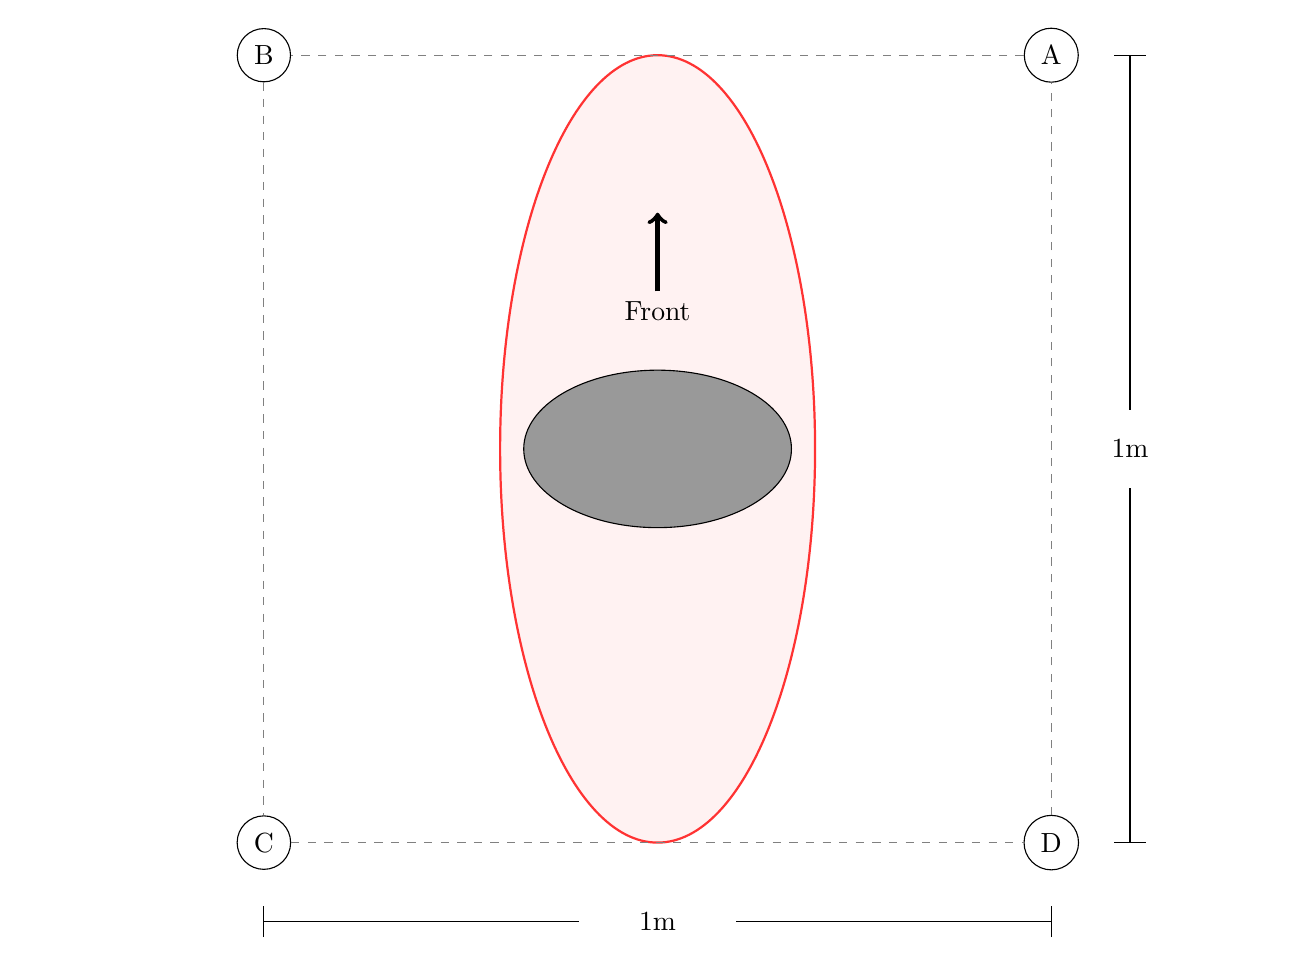
\begin{tikzpicture}[node distance=2cm]

\draw[help lines] (-5,-5) (5,5);

\node[hydrophone] (A) at (5,5)   {A};
\node[hydrophone] (B) at (-5,5)  {B};
\node[hydrophone] (C) at (-5,-5) {C};
\node[hydrophone] (D) at (5,-5)  {D};

% Draw the kayak
\draw[color=red!80,fill=red!5, thick] (0,0) ellipse (2 and 5);
\draw[fill=black!40] (0,0) ellipse (1.7 and 1);
\draw[->,ultra thick] (0,2) -- (0,3);
\node[below] at (0,2) {Front};

% Draw lines to hydrophones
\draw[color=gray,dashed]
	(A) -- (B)
	(B) -- (C)
	(C) -- (D)
	(D) -- (A)	
;

% Draw the measurements
\draw[]
	(6,0.5)  -- (6,5)    % vertial line
	(6,-0.5) -- (6,-5)   % vertial line
	(5.8,5)  -- (6.2,5)  % horizontal tick
	(5.8,-5) -- (6.2,-5) % horizontal tick
	
	(-5,-6)   -- (-1,-6)    % horizontal line
	(1,-6)    -- (5,-6)     % horizontal line
	(-5,-6.2) -- (-5,-5.8)  % vertical tick
	(5,-6.2)  -- (5,-5.8)   % vertical tick
;
\node[] at (6,0)  {1m};
\node[] at (0,-6) {1m};

% to center image (offsets measurement line on right)
\path[fill=none] (-8,0) (8,0);

\end{tikzpicture}
\end{center}
\caption{The hydrophone array attached to the kayak.}
\label{fig:array}
\end{figure}


%%%%%%%%%%%%%%%%%%%%%%%%%%%%%%%%%%%%%%%%%%%%%%%%%%%%%%%%%%%%%%%%%%%%%%%%%%%%%%%
\section{Software Setup}

\subsection{Loading Software}

\subsection{Configuring Settings}

\end{document}

